\documentclass[a4paper, 12pt]{article}

\usepackage{escexam}

%\excludecomment{solution}

%\renewcommand*\ttdefault{cmvtt}
\setlength{\headheight}{80.05003pt}

\begin{document}

%\vspace*{14ex}

\makeheader{1}                              					% examination number (used to set theorem, lemma numbers)
           {September 2, 2022}      					         		% examination date or deadline
					 {40}											% total marks
					 {Homework Assignment 2}							% Minor Quiz 1, Major Quiz 2, End sem, etc
					
\begin{tabular}{cl}
1. & Write the answers \textbf{neatly} in the given boxes.\\
2. & You may  discuss the solutions with the other students, but you have to write them in your own words.\\
%4. & Do not give derivations/elaborate steps unless the question specifically asks you to provide these.
\end{tabular}


\begin{problem}{}
(10 points)  Construct a timed automation model of a thermostat where the heater will be switched on when the room temperature is less than 22C and switched off when the temperature is above 26 Celsius. We also have the following additional requirement. Before switching on or off, it will generate a ``beep'' sound every second for 5 seconds as a warning. That means once the system senses that the temperature is less than 22C, it will generate the warning first, and then the heater will be switched on. Similarly, a warning sound will be issued before switching off the heater after the temperature reaches 26C.


\noindent
\\
\\
\begin{minipage}{1\textwidth}
		\rectangle{\linewidth}{19cm}
		% \ruledrectangle{7}
\end{minipage}

\newpage
\ \\
\begin{minipage}{1\textwidth}
		\rectangle{\linewidth}{24cm}
		% \ruledrectangle{7}
\end{minipage}
\newpage
\ \\
\begin{minipage}{1\textwidth}
		\rectangle{\linewidth}{24cm}
		% \ruledrectangle{7}
\end{minipage}
\newpage
\ \\
\begin{minipage}{1\textwidth}
		\rectangle{\linewidth}{24cm}
		% \ruledrectangle{7}
\end{minipage}
\end{problem}


\newpage
\begin{problem}{}
(10 points)
Consider the following protocol that ensures mutual exclusion among N processes
using real-time clocks and a shared variable $\texttt{lock}$.

Initially $\texttt{lock}$ is 0.

Every process follows the following process:

\begin{verbatim}
   loop
      wait until lock = 0;
      wait for a delay <= 2;
      set lock to process id;
      wait for a delay >= 3;
      if lock = process id 
      	enter critical section;
      go back to the wait state     
   end
\end{verbatim}
Draw a timed automaton to capture the behavior of a process that follows the protocol.

\noindent
\\
\\
\begin{minipage}{1\textwidth}
		\rectangle{\linewidth}{16cm}
		% \ruledrectangle{7}
\end{minipage}
\newpage
\ \\
\begin{minipage}{1\textwidth}
		\rectangle{\linewidth}{24cm}
		% \ruledrectangle{7}
\end{minipage}
\newpage
\ \\
\begin{minipage}{1\textwidth}
		\rectangle{\linewidth}{24cm}
		% \ruledrectangle{7}
\end{minipage}
\newpage
\ \\
\begin{minipage}{1\textwidth}
		\rectangle{\linewidth}{24cm}
		% \ruledrectangle{7}
\end{minipage}
\end{problem}


\newpage
\begin{problem}{}
(10 points) Construct an equivalent flat FSM giving the semantics of the hierarchy. Describe
in words the input/output behavior of this machine. \\
\begin{figure}[h]
\begin{center}
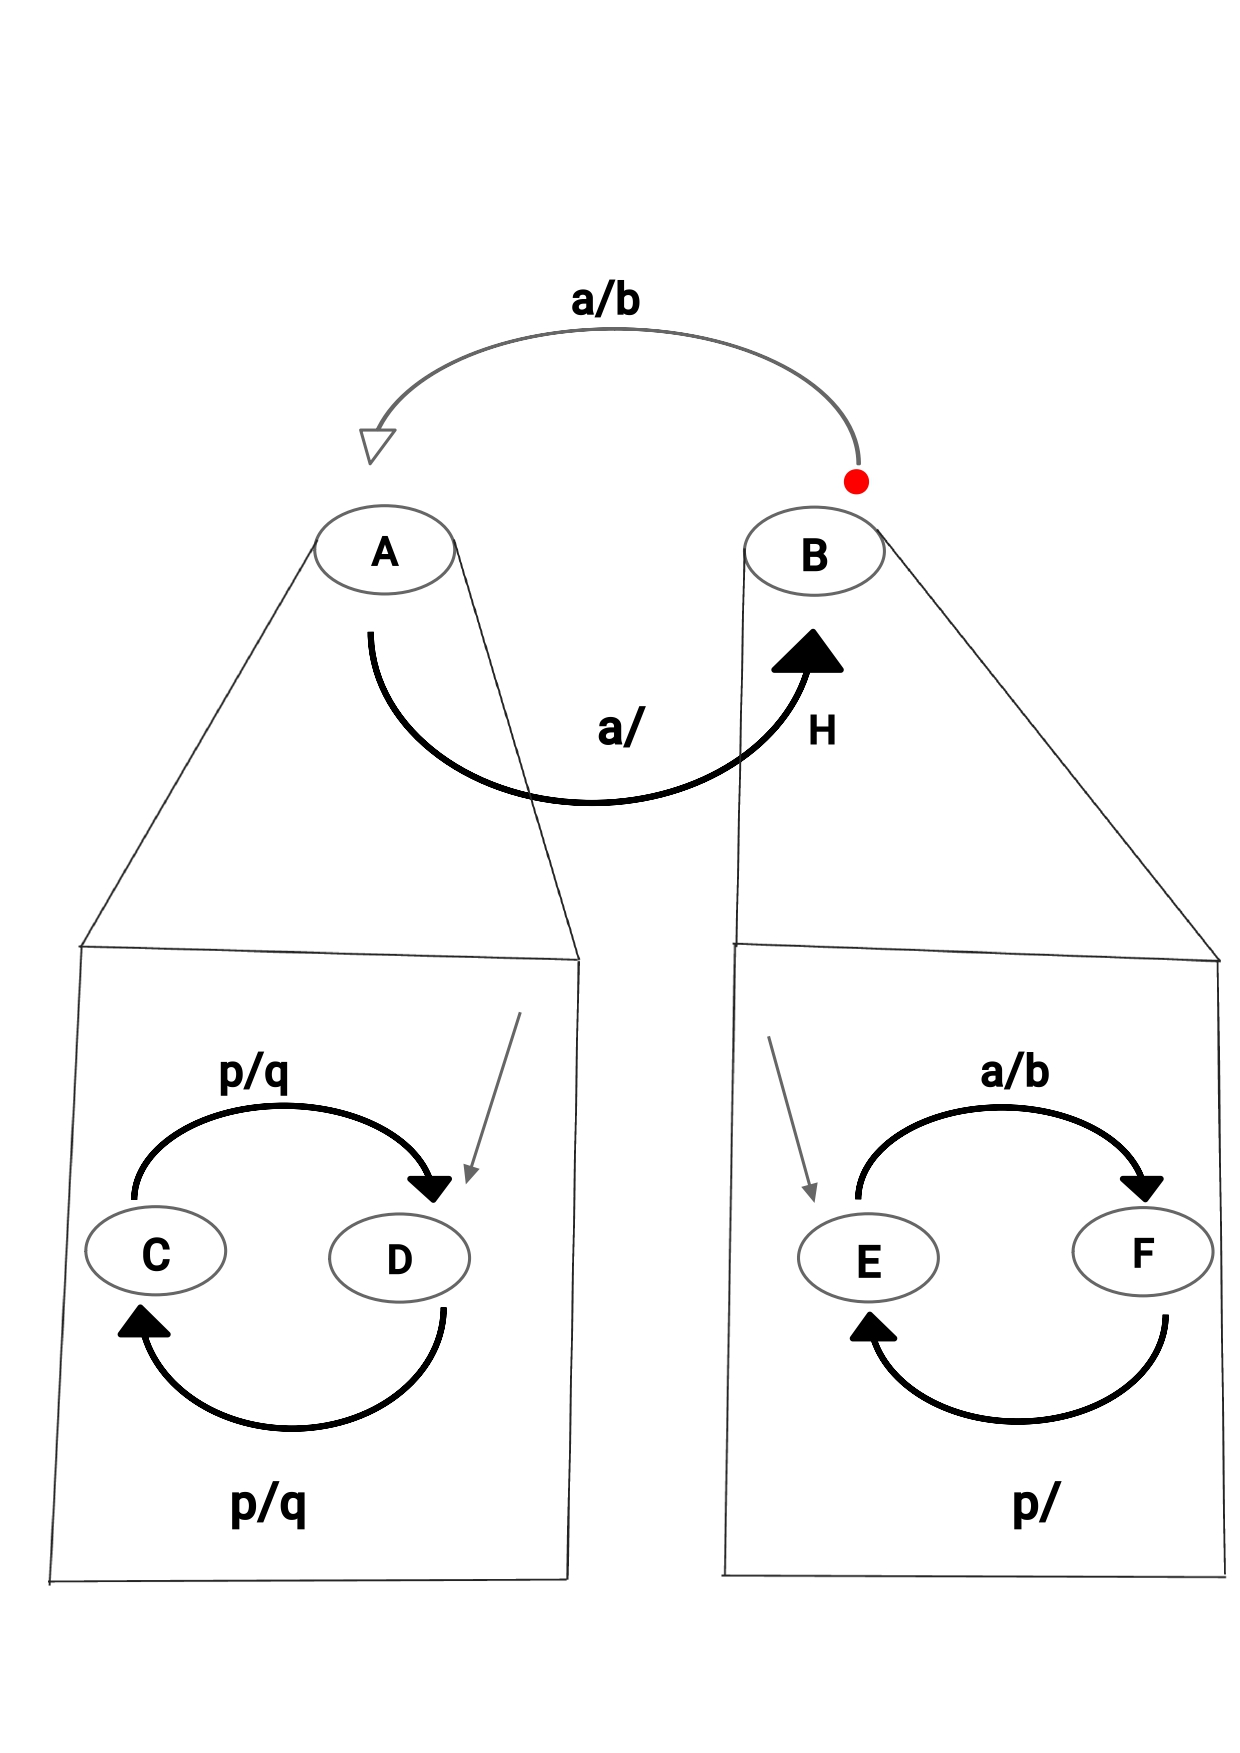
\includegraphics[width=7cm]{image.jpg}
\end{center}
\end{figure}



\noindent
\\
\\
\begin{minipage}{1\textwidth}
		\rectangle{\linewidth}{13cm}
		% \ruledrectangle{7}
\end{minipage}
\newpage

\ \\
\begin{minipage}{1\textwidth}
		\rectangle{\linewidth}{24cm}
		% \ruledrectangle{7}
\end{minipage}
\newpage
\ \\
\begin{minipage}{1\textwidth}
		\rectangle{\linewidth}{24cm}
		% \ruledrectangle{7}
\end{minipage}
\newpage
\ \\
\begin{minipage}{1\textwidth}
		\rectangle{\linewidth}{24cm}
		% \ruledrectangle{7}
\end{minipage}
\end{problem}



\newpage
\begin{problem}{}
(10 points) Problem 8 in the Exercises of Chapter 6 in [LS15].

\noindent
[LS15] Edward A. Lee and Sanjit A. Seshia, Introduction to Embedded Systems, A Cyber-Physical Systems Approach, Second Edition, http://LeeSeshia.org, ISBN 978-1-312-42740-2, 2015. \\
\\
\begin{minipage}{1\textwidth}
		\rectangle{\linewidth}{23cm}
		% \ruledrectangle{7}
\end{minipage}
\newpage
\ \\
\begin{minipage}{1\textwidth}
		\rectangle{\linewidth}{24cm}
		% \ruledrectangle{7}
\end{minipage}
\newpage
\ \\
\begin{minipage}{1\textwidth}
		\rectangle{\linewidth}{24cm}
		% \ruledrectangle{7}
\end{minipage}
\newpage
\ \\
\begin{minipage}{1\textwidth}
		\rectangle{\linewidth}{24cm}
		% \ruledrectangle{7}
\end{minipage}
\end{problem}

\end{document}